
Below we describe the simulation studies performed to evaluate the impact of the de-scoping options we identified on the three 
science drivers. We  first compare each change individually to the performance of the reference configuration, and then study
a select set of changes in combination to evaluate their combined effect on the physics performance. For each option we 
describe the simulations employed, ranging from generator level evaluations of count rates to single particle and single jet
\geant simulations + reconstruction to full \hijing central Au+Au \geant simulations and reconstruction. All studies were 
performed for 200 GeV Au+Au collisions.
\section{Hadronic calorimeter changes}
\subsection{Outer HCal thinning}
The main impact on the science program from thinning the outer HCal is expected in areas:
\begin{itemize} 
\item Reduced jet energy containment leading the larger systematic uncertainties in the jet energy scale and larger fluctuations
in the jet-by-jet energy measurement.
\item Increased punch-through of high momentum particles leading to a fragmentation function bias
\end{itemize}
The impact was studied with full \geant simulations and jet reconstruction using the \antikt algorithm for single jets 
for the reference configuration (outer radius 260~cm), the thinned oHCal (outer radius 240~cm) and the minimal outer HCal needed 
to serve as flux return (outer radius 220~cm). 

\begin{figure}[hbt]
  \centering
  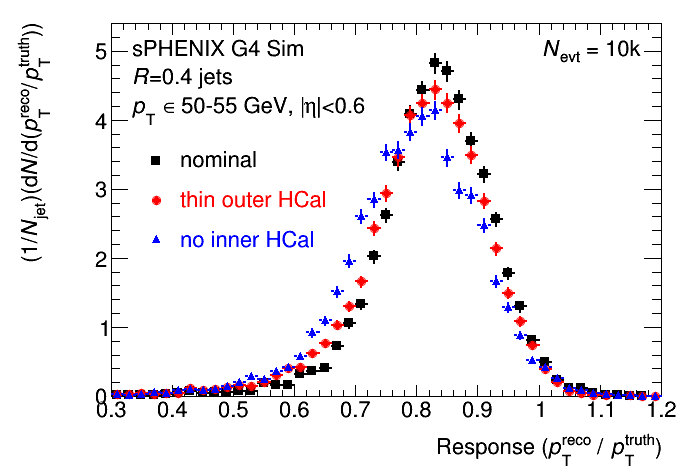
\includegraphics[width=0.45\linewidth]{figs/jetresponse_thinhcal}
  \hspace{0.05\linewidth}
  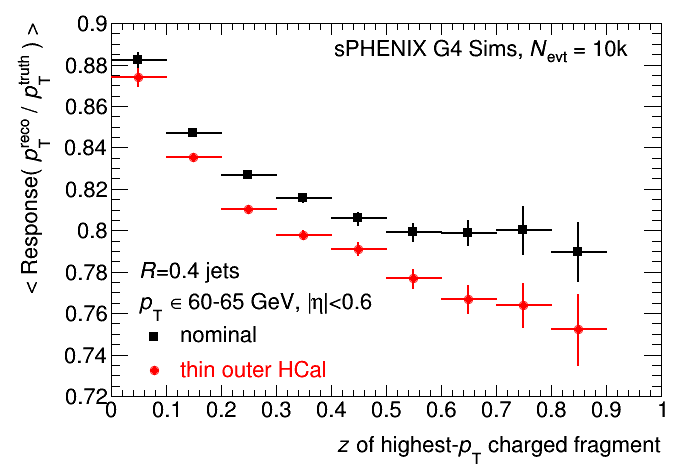
\includegraphics[width=0.45\linewidth]{figs/fragmentation_bias_thinhcal}
  \caption{(Left) Comparison of the jet response for three different HCal configurations: Nominal outer HCal (black markers), 
   outer HCal thinned by 20~cm (red markers) and no inner HCal (blue markers). 
   (Right) Comparison of the jet fragmentation bias for nominal (black markers) and thinned outer HCal (240~cm outer radius, red markers).}
  \label{fig:jet_energy_scale_thin_hcal}
\end{figure}
\paragraph{Jet energy response}
Figure~\ref{fig:jet_energy_scale_thin_hcal}(left) shows the energy
response, $p_T^{reco}/p_T^{truth}$, of the calorimeter system to high
\pT jets for three calorimeter configurations: the nominal outer HCal
thickness (outer radius = 260~cm), an outer HCal thinned by about one
interaction length (outer radius = 240~cm) and nominal outer HCal and
EMCal, but no inner HCal (blue markers). The simulations show only a
small loss in total energy containment for the thinned outer HCal
configuration relative to the nominal configuration, combined with a
moderate increase in the number of jets for which less than 70\% of
the energy was reconstructed.  Further studies showed that the change
in the jet response only has a small effect on reconstructing unfolded
jet spectra, even when uing a Gaussian kernel that ignores the
increases low-energy tail. Removing the inner HCal has a significantly
larger effect on the mean and shape of the jet response.

\paragraph{Fragmentation function bias} 
One expects that the thinned HCal configuration leads to the biggest
change in jet response for jets with high-z fragmentation products
that are not contained in the calorimeter system. To study this
effect, we plot the average jet energy response $\langle
p_T^{reco}/p_T^{truth}\rangle$ as a function of the momentum fraction
$z$ carried by the highest \pt charged fragment in
Fig.~\ref{fig:jet_energy_scale_thin_hcal}(right). Even for the nominal
HCal configuration, a dependence of the response on the hardness of
the jet fragmentation is seen, with a change of about 0.08 in $\langle
p_T^{reco}/p_T^{truth}\rangle$ from softest to hardest fragmenting
jets.  For the thinned HCal configuration, this increases to
0.11-0.13. We expect that this additional bias would only lead to a
moderate increase in the uncertainty of fragmentation function ratios
for Au+Au/p+p, as the increase is only about 50\% of the bias already
seen in the nominal configuration, and present in both p+p and Au+Au
events (i.e., only related to the single particle containment).


\subsection{Outer HCal shortening}

For the shortened outer HCal (reducing the pseudorapidity coverage
from $|\eta| < 1.1$ to $|\eta| < 0.9$), all measured at the outer
corner of the calorimeter) the expected impact is in the statistics of
jet related probes. The reduction in coverage will predominantly
affect lower \pt jets, as jets at the highest \pT have a narrow
rapidity distribution that falls within the remaining acceptance.
\begin{figure}[hbt]
  \centering
  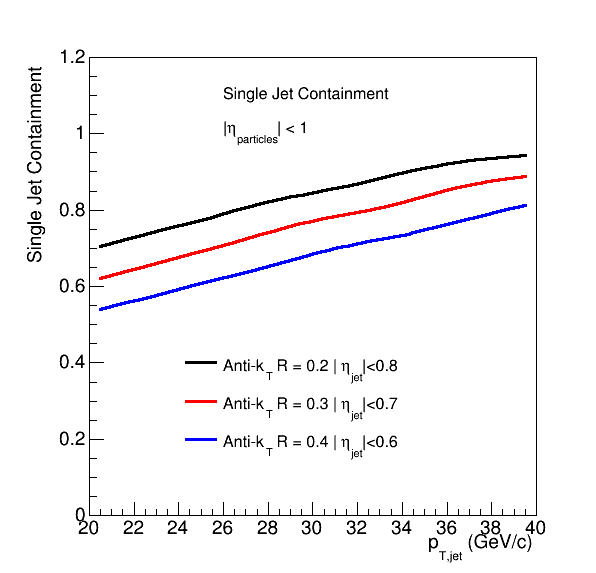
\includegraphics[width=0.4\linewidth]{figs/SingleJet_eta_reference}
  \hspace{0.1\linewidth}
  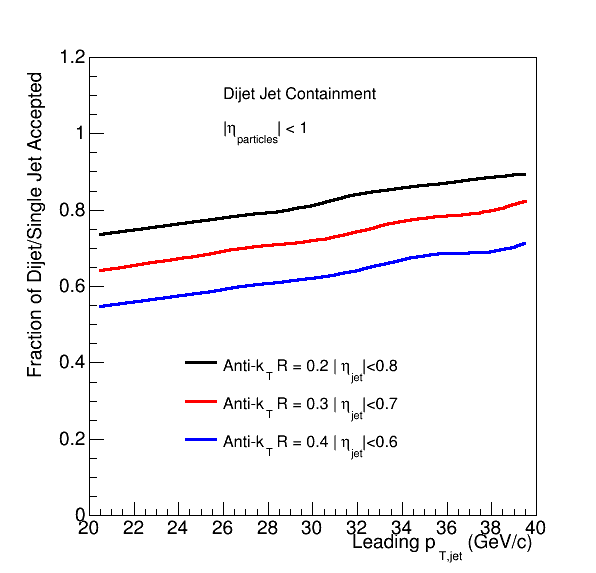
\includegraphics[width=0.4\linewidth]{figs/Dijet_eta_reference}
  \caption{(Left) 
  Fraction of jets fully contained within the acceptance of the nominal calorimeter system as a function
  of jet \pt, for three different jet radius parameters, R = 0.2 (black), R=0.3 (red) and R=0.4 (black). 
   (Right) 
  Fraction of dijets with both jets fully contained within the acceptance of the nominal calorimeter system as a function
  of jet \pt, for three different jet radius parameters, R = 0.2 (black), R=0.3 (red) and R=0.4 (black).}
  \label{fig:jet_containment_nominal}
\end{figure}
Figure~\ref{fig:jet_containment_nominal} shows the fraction of jets (left) and dijets (right) contained in the nominal calorimeter 
system as a function of jet \pt, obtained from generator level distributions. As expected, the fraction of fully contained jets is lowest for low \pT jets (which have a wider
rapidity distribution) than for hight \pt jets. The difference between the nominal length outer HCal and the shortened outer HCal
is well approximated by the difference between the black and blue curves shown in the figures.

Some of the physics impact can be recovered using tracker + EMCal reconstruction of jets, although reduced control over the jet 
energy scale and increased jet-by-jet fluctuations will limit the precision that can be achieved with such studies.

\subsection{Removal of the inner HCal}

As shown in Fig.~\ref{fig:jet_energy_scale_thin_hcal}(left), the impact on jet energy scale and fluctuations for this option is 
found to be significantly larger than for the thinned outer HCal option. 
with major impact on engineering of the inner detector mechanical design leading to expectations of minimal overall savings.
We therefore did not perform detailed studies of this option.

\section{EMCal}
\subsection{Changing EMCal segmentation}
\subsubsection{2$\times$2 ganging of EMCal channels}
The reduced EMCal segmentation from 2x2 ganging of readout channels is expected to affect three physics areas: jet finding 
and jet energy reconstruction, electron/hadron separation for the $\Upsilon$ to $e^+ e^-$ channel and photon identification.
We performed full \geant and reconstruction studies of the effect on the single jet response and full \geant simulations for 
Au+Au \hijing events for electron identification. Studies of the effect on photon identification are ongoing.

\paragraph{Effect on jet energy response}
\begin{figure}[hbt]
  \centering
  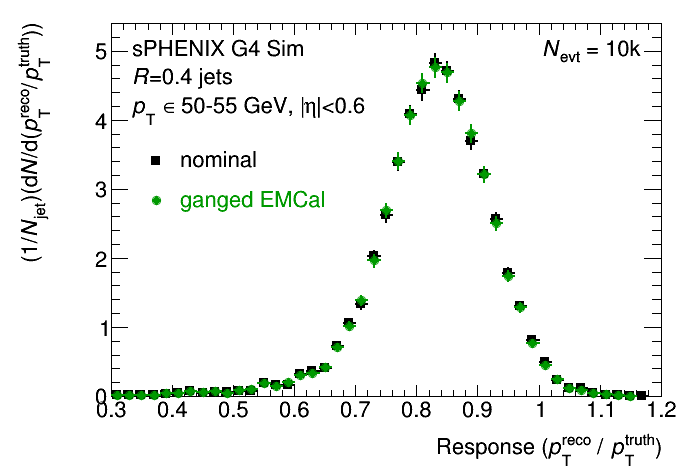
\includegraphics[width=0.4\linewidth]{figs/jetresponse_ganged_ecal}
  \hspace{0.1\linewidth}
  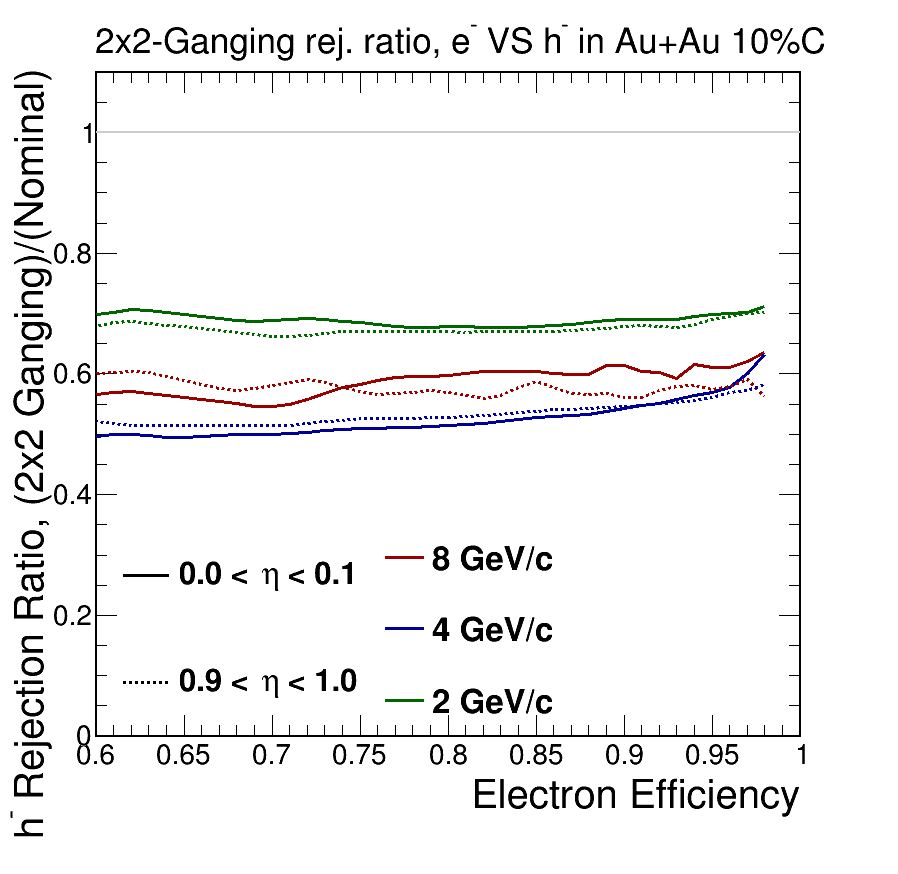
\includegraphics[width=0.4\linewidth]{figs/hadron_rejection_ganged_over_nominal}
  \caption{(Left)
  Jet response for the nominal calorimeter systems (black markers) and the calorimeter system with ganged EMCal readout 
(green markers) for high \pt jets.
   (Right)
  Ratio of the hadron rejection factor as a function of electron efficiency between the ganged EMCal configuration 
and the nominal EMCal configuration, for central Au+Au collisions. The ratio is shown for two pseudorapidity regions 
and three particle momenta. }
  \label{fig:jet_containment_ganged}
\end{figure}
Figure~\ref{fig:jet_containment_ganged}(left) shows the energy response in the calorimeter system for high \pt jets for the 
nominal configuration (black markers) and the ganged EMCal configuration (green markers). Ganging has no visible effect
on this distribution, as the change in granularity is small compared to the typical jet size and the total collected
jet and background energies are unchanged.

\begin{figure}[hbt]
  \centering
  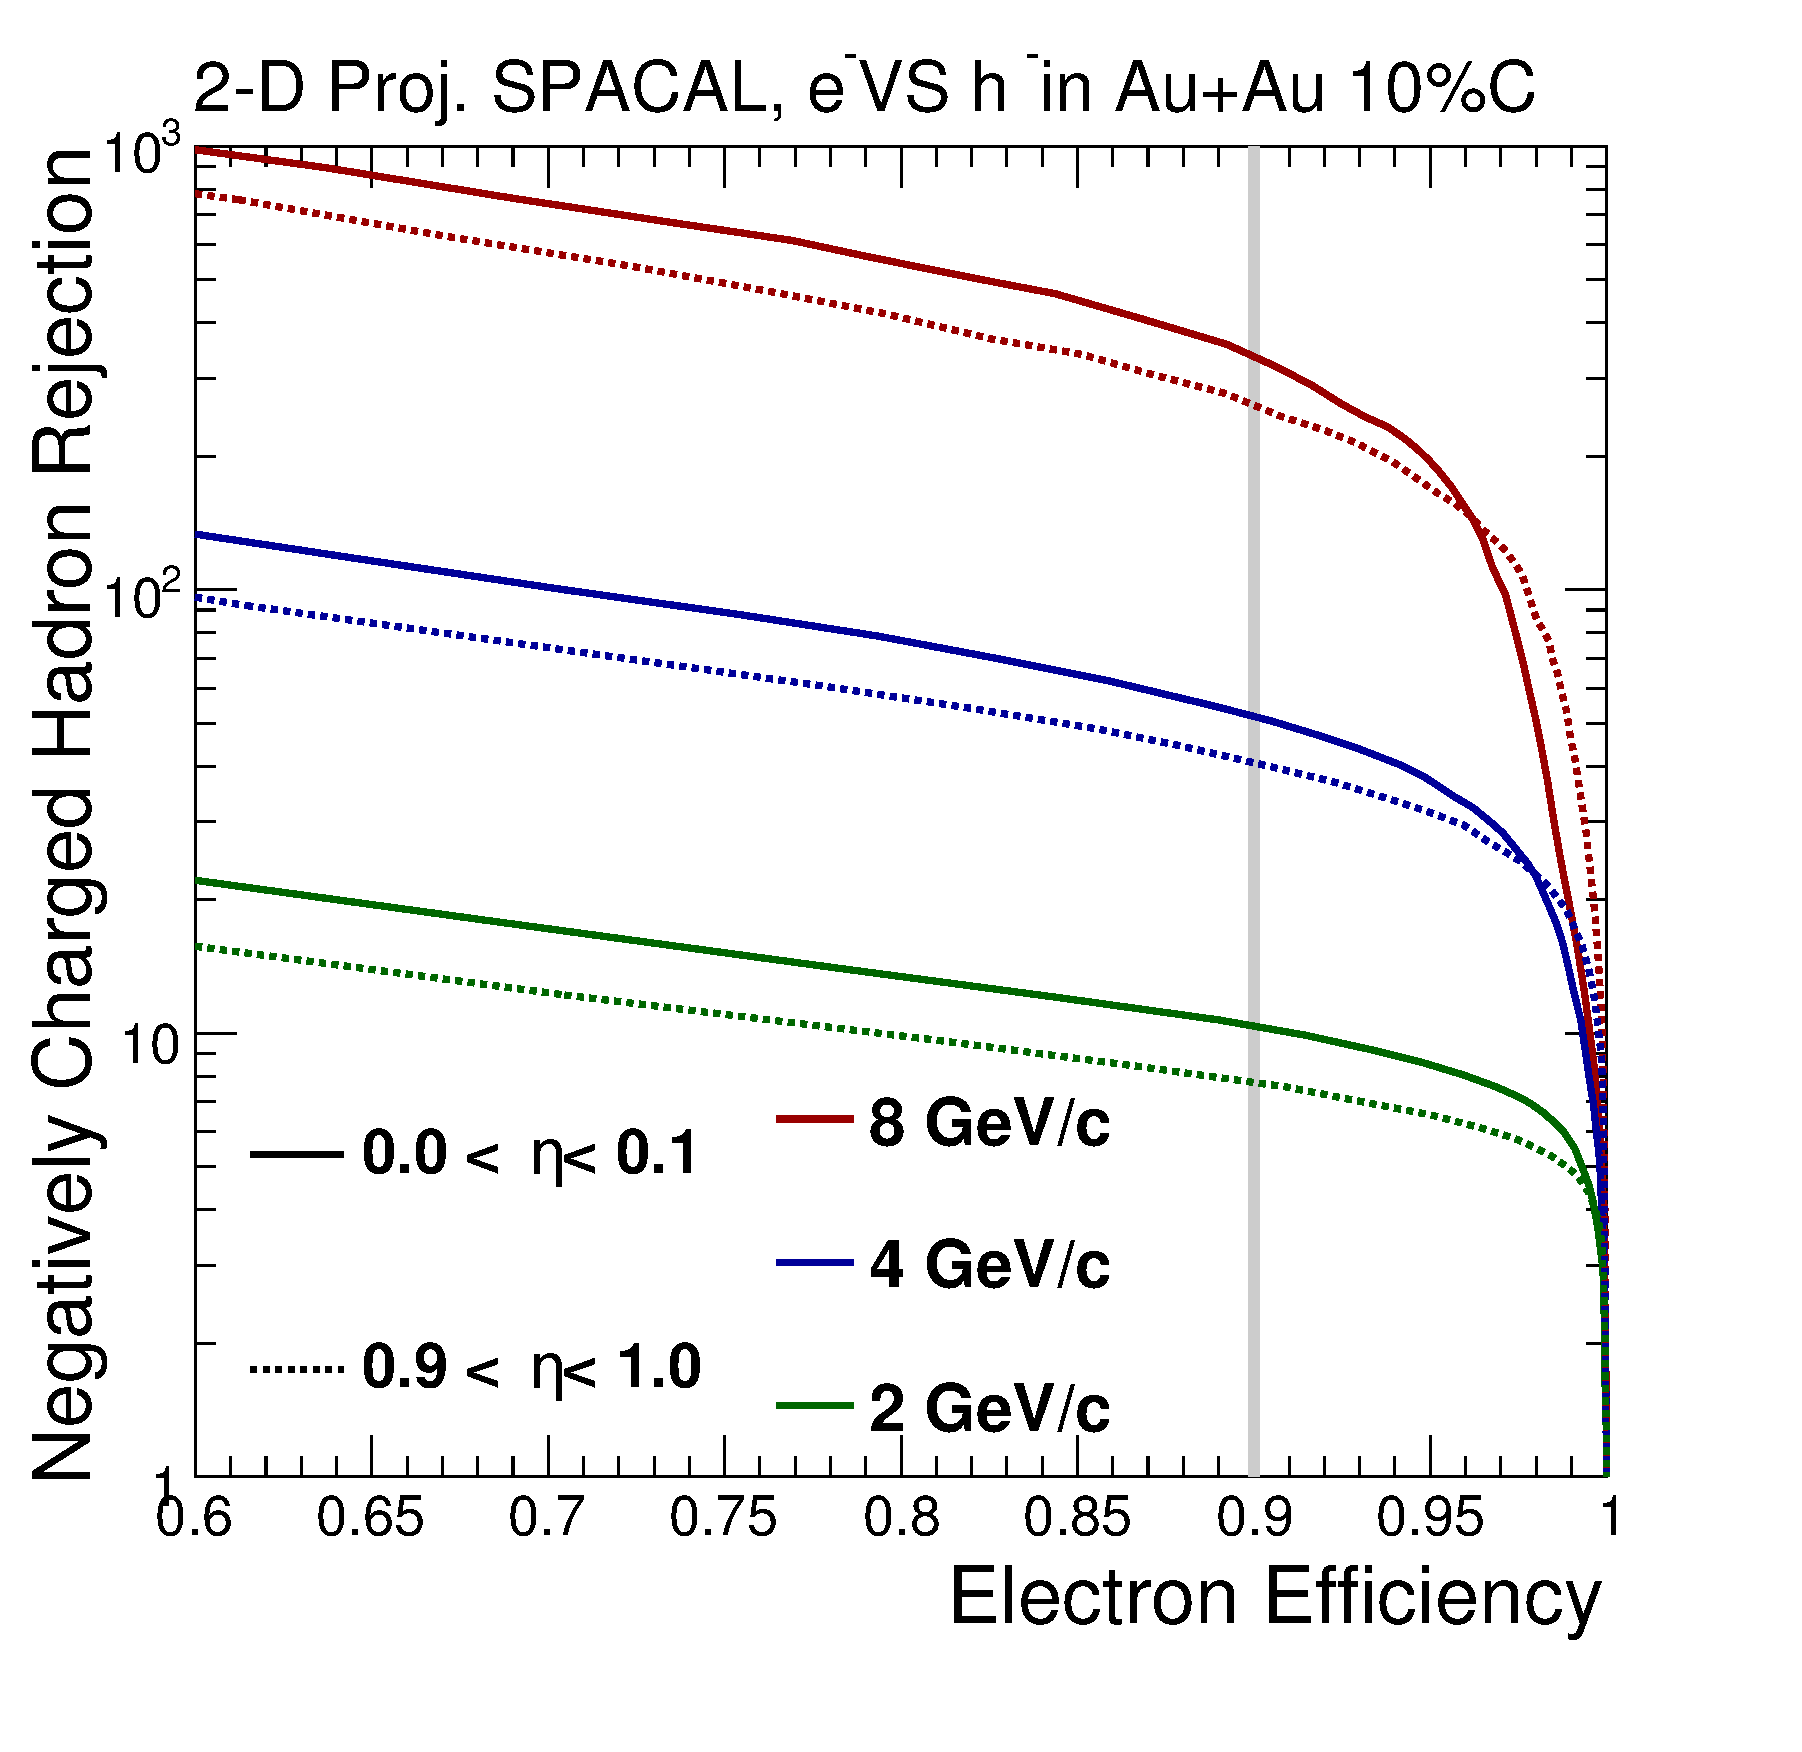
\includegraphics[width=0.4\linewidth]{figs/DrawEcal_Likelihood_Sum_RejectionCurve_AuAuSummary}
  \hspace{0.1\linewidth}
  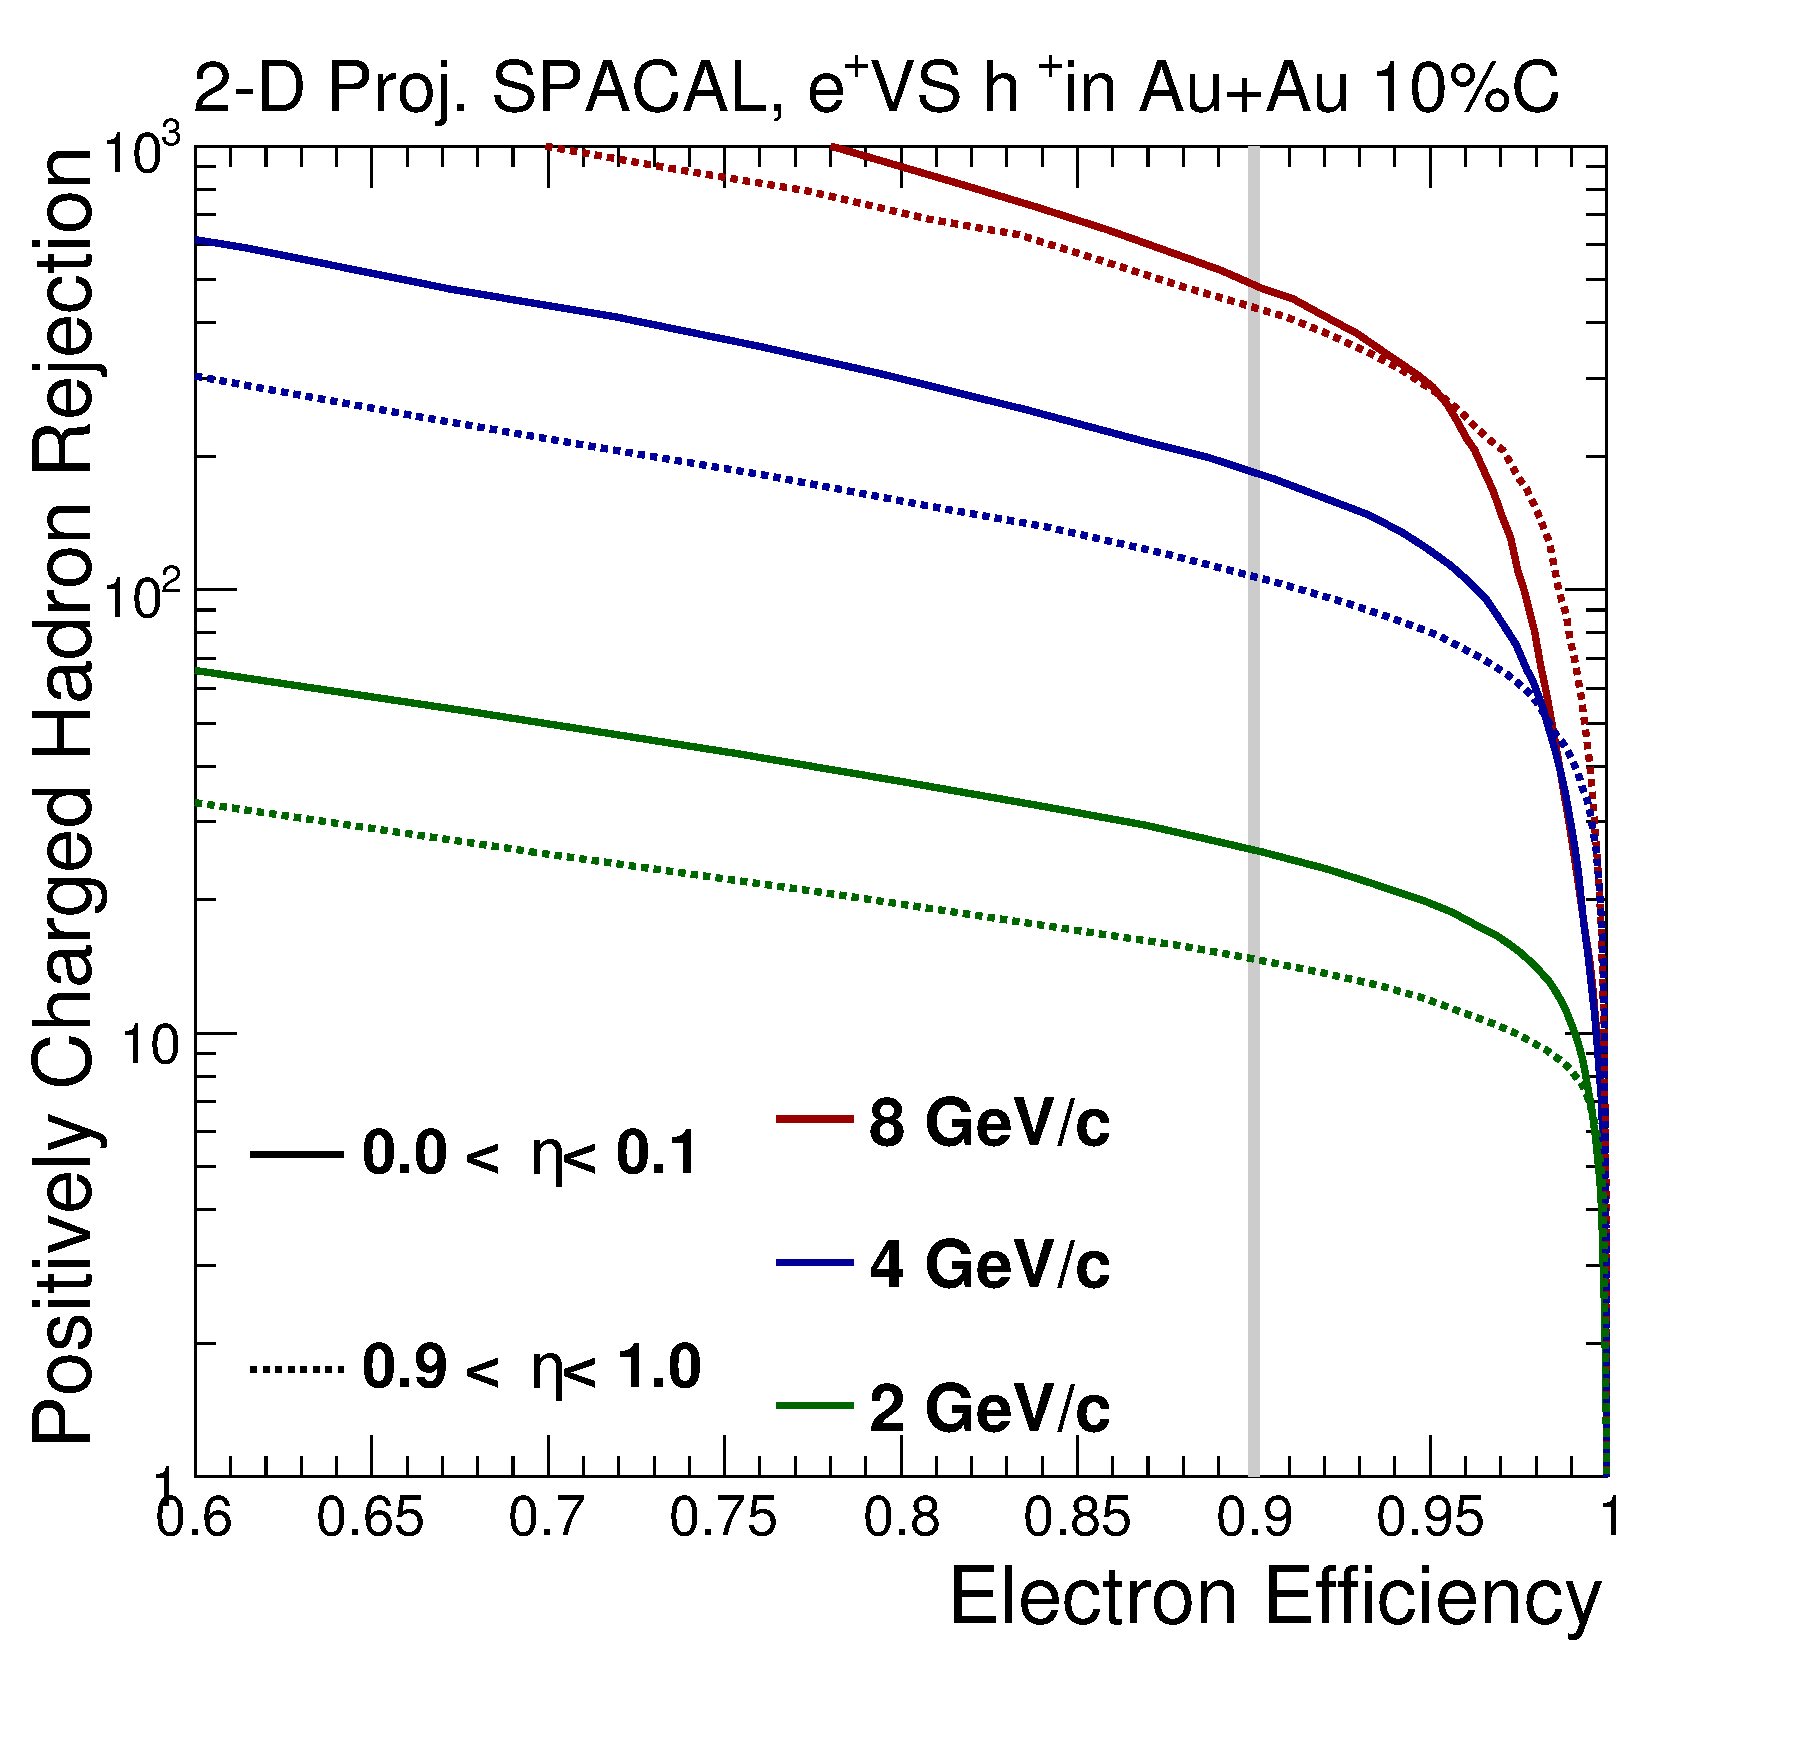
\includegraphics[width=0.4\linewidth]{figs/DrawEcal_Likelihood_Sum_RejectionCurve_AuAuSummaryPos}
  \caption{For a $2\times2$ ganged EMCal (with inner HCal present)
    inclusive charged hadron rejection is plotted on the left (right)
    as function of electron ID efficiency, for negatively (positively)
    charged tracks of three choices of momentum and for middle and
    edge rapidity in 10\% most central Au+Au events.}
  \label{fig:eid_auau}
\end{figure}

\paragraph{Effect on electron/hadron separation}

The hadron rejection factors for the $2\times 2$ EMCal readout ganging
were obtained for \hijing simulations of central Au+Au collisions, and
are shown for negative (left) and positive (right) hadrons as a
function of electron efficiency in Fig.~\ref{fig:eid_auau}.  The
relative change compared to simulations of the nominal EMCal
configuration can be seen in
Fig.~\ref{fig:jet_containment_nominal}(right), which shows the ratio
of the hadron rejection factor between the ganged configuration and
the nominal configuration as a function of electron efficiency for
central Au+Au collisions. The change in rejection factor ranges from
0.7 for low \pt hadrons at central rapidity to 0.5 for intermediate
\pt hadrons at central rapidity. Simulations of the current nominal
EMCal configuration show a rejection factor of about 200 for the
kinematic range relevant for $\Upsilon$ identification at 70\%
electron efficiency. This rejection factor for the nominal
configuration is twice as large as that assumed for $\Upsilon$ studies
in the pCDR. The loss in rejection by a factor of two for the ganged
configuration is significant, but will still allow the $\Upsilon$
program as discussed in the pCDR, albeit with a reduced safety margin.

\subsubsection{Increasing EMCal tower size}
The reduced EMCal segmentation from increasing the tower dimensions
from $d\eta \times d\phi = 0.024 \times 0.024$ to $0.033 \times 0.28$
was not evaluated with full \geant simulations, as time did not permit
implementing the corresponding detector geometry. However, as the
change increases the tower area by 60\%, as compared to a factor of
four for the 2x2 ganging, the expected impact can be well estimated
based on the 2x2 ganging full simulations. For the jet response, the
2x2 ganging did not show any noticable effect, implying that the 60\%
increased tower size will also have no effect on jets. For $e/h$
separation, the effect of the 2x2 ganging of about a factor of two
suggests scaling with the $\sqrt{\mbox{area}}$, i.e., the fluctuations
in the background energy. This implies a 26\% change in $e/\pi$
separation in central Au+Au collisions for the 60\% increase in tower
size, which is well within the projected safety margin for the
measurement.

\subsection{Reduced EMCal pseudorapidity coverage}
Reducing the EMCal coverage to $\| \eta \| < 0.6$ will directly affect
the expected statistics for $\Upsilon$ to $e^+ e^-$ and photon-based
measurements. The corresponding loss in statistics is summarized in
the table below, based on generator level studies. For jet
measurements, the reduced coverage leads to a change in jet response
across the EMCal boundary. This effect was evaluated by full \geant
simulations and reconstruction of the single jet response in different
regions of pseudorapidity and jet \pt.

\paragraph{Loss of $\Upsilon$ acceptance}
\begin{figure}[hbt]
  \centering
  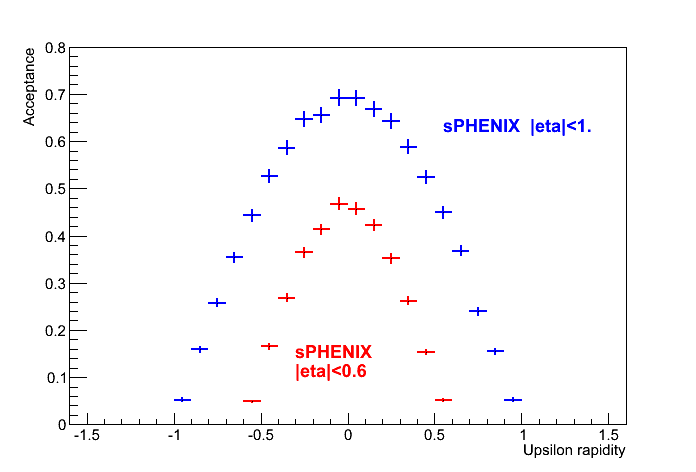
\includegraphics[width=0.4\linewidth]{figs/upsilon_rate_y}
  \hspace{0.1\linewidth}
  \includegraphics[width=0.4\linewidth]{figs/upsilon_rate_pT}
  \caption{(Left)
  $\Upsilon$ to $e^+ e^-$ acceptance as a function of rapidity for the nominal (blue markers) and $\| \eta \| < 0.6$ configurations,
  averaged over $\Upsilon$ \pt. 
  (Right) $\Upsilon$ to $e^+ e^-$ acceptance as a function of $\pt$ for the nominal (blue markers) and $\| \eta \| < 0.6$ 
  configurations, averaged over $\eta$.}
  \label{fig:upsilon_rate}
\end{figure}

Figure~\ref{fig:upsilon_rate} shows the acceptance for $\Upsilon$ to $e^+ e^-$ decays for the nominal and reduced $\eta$ EMCal
configurations as a function of rapidity (left) and $\pt$ (right). The figures suggest a loss of about 60\% of overall 
$\Upsilon$ statistics, with the largest effect at low \pt. In $\Upsilon$ rapidity, about 0.5 units in rapidity reach are 
lost when requiring equal $\Upsilon$ statistics for nominal and reduced $\eta$ configurations.

\paragraph{Change in jet response} 
\begin{figure}[hbt]
  \centering
  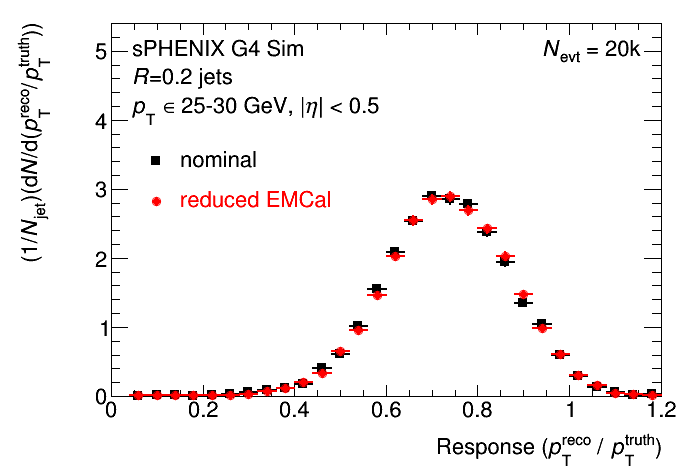
\includegraphics[width=0.4\linewidth]{figs/jet_response_reduced_emcal_eta_0} 
  \hspace{0.1\linewidth}
  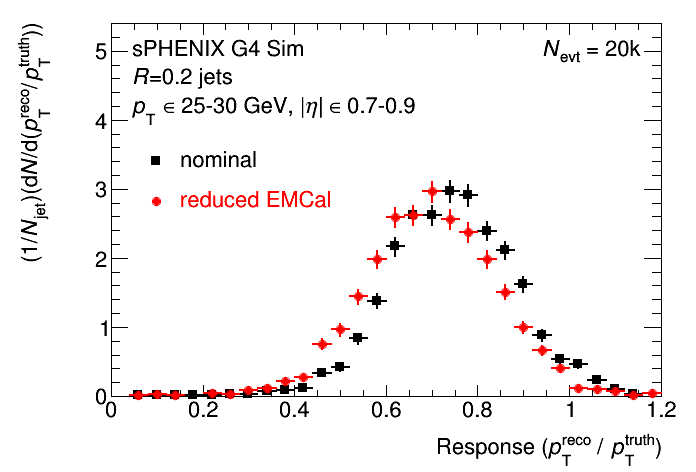
\includegraphics[width=0.4\linewidth]{figs/jet_response_reduced_emcal_eta_07}
  \caption{(Left) Comparison of jet response for $|\eta| <  0.5$ jets for nominal (black markers) and reduced acceptance (red markers) EMCal configuration.
  (Right) Comparison of jet response for $|\eta| > 0.5$ jets for nominal (black markers) and reduced acceptance (red markers) EMCal configuration.}
  \label{fig:jet_response_reduced_emcal}
\end{figure}

The effect of reducing the EMCal acceptance to $|\eta| < 0.6$ on the
jet energy response, $p_T^{reco}/p_T^{truth}$, was studied for low \pt
jets, where we expect the largest effect, for three regions of jet
pseudorapidity, $|\eta| < 0.5$
(Fig.\ref{fig:jet_response_reduced_emcal}, left), $0.5 < |\eta| < 0.7$
(not shown) and $|\eta| > 0.7$
(Fig.~\ref{fig:jet_response_reduced_emcal}, right). As expected,
essentially no change is observed for the central rapidity region,
while for $|\eta| > 0.7$ a shift in the mean of several percent and
the appearance of an enhanced low response tail are
apparent. Experience at LHC suggest typical best-case jet response
uncertainties of 2--3\%. Assuming an uncertainty in the correction of
the reduced response at large $\eta$ of 50\% or better, the changed
response compared to the nominal configuration will lead to a
significant, but still tolerable increase in unfolding uncertainties
for jet spectra.

\begin{figure}[hbt]
  \centering
  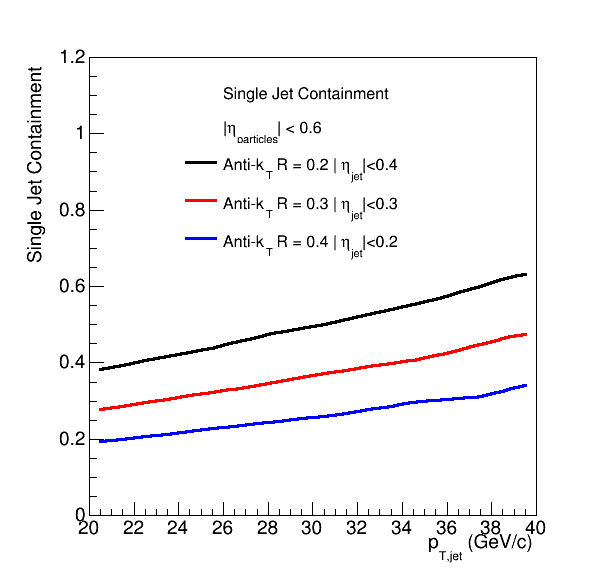
\includegraphics[width=0.4\linewidth]{figs/SingleJet_eta_ecal06}
  \hspace{0.1\linewidth}  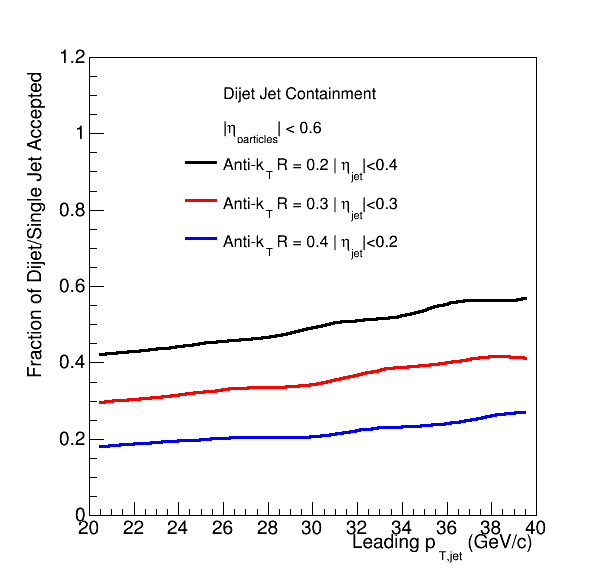
\includegraphics[width=0.4\linewidth]{figs/Dijet_eta_ecal06}
  \caption{(Left)
  Fraction of jets fully contained within the acceptance of the $|\eta| < 0.6$ EMCal configuration as a function
  of jet \pt, for three different jet radius parameters, R = 0.2 (black), R=0.3 (red) and R=0.4 (black).
   (Right)
  Fraction of dijets with both jets fully contained within the acceptance of $|\eta| < 0.6$ configuration as a function
  of jet \pt, for three different jet radius parameters, R = 0.2 (black), R=0.3 (red) and R=0.4 (black).}
  \label{fig:jet_containment_reduced_emcal}
\end{figure}

We also investigated the loss in statistics when requiring jets and dijets to be fully contained in the reduced EMCal acceptance. The result is shown 
in Fig.~\ref{fig:jet_containment_reduced_emcal}, to be compared with the acceptance for the nominal 
configuration shown in Fig.~\ref{fig:jet_containment_nominal}. One observes that for low \pt dijets, this requirement leads to a loss of dijet
statistics by a factor of 2-3, depending on the selected jet radius parameter $R$.

\section{Outer tracker}

For the outer tracker, the performance of a TPC tracker was evaluated using \geant simulations of single particles, single $\Upsilon$ to $e^+ e^-$
decays, and full \hijing and \geant simulations in a limited acceptance around mid-rapidity (due to timing limitations). Simulations were performed
for an ideal TPC and two configurations with inner field cage boundary at $r=20$~cm and $r=30$~cm. For the latter configurations, effects of 
residual space charge distortions expected after corrections were included. We evaluated general performance characteristics (efficency, fake track

rate, DCA and momentum resolution) and specifically the $\Upsilon$ mass resolutions for the different cases. The TPC simulations were performed
in combination with the 3-layer MAPS configuration of the reference design, and include the effects of track reconstruction and kinematic fits. 
The effect of various inner tracker options on the tracking performance is evaluated separately in \ref{sec:innertracker}.

\subsection{Studies of $\Upsilon$ mass resolution}

We have performed TPC simulations with and without residual space charge distortions
(i.e., after corrections)  and for readout of 60 and 30 TPC layers, for a field cage configuration with 20~cm inner radius and 78~cm outer radius 
in all cases. The space charge distortions are calculated follow the prescriptions outlined in the ALICE TDR and 
specifically the results from the thesis of Rossiger.  We use a second order Langevin equation to 
swim particles through the static electric and magnetic fields producing a pair of distortion results $dr(r,z)$ and $rd{\phi}(r,z)$.  
Our calculations are normalized to ALICE gas conditions (Ne, CO2 90:10) and reproduce well the distortion in the ALICE TDR.  

For simplicity, we have assumed that post-correction errors due to space charge distortions will be linearly proportional to the amount of the 
distortion itself.  These errors are modeled as two portions, labelled as "accuracy" and "precision".  Errors in accuracy will move points 
in a correlated fashion due to either over- or under-correcting the distortion.  In meetings with ALICE, they quoted a 1 mm accuracy 
after a correction of 20 cm.  Errors in precision are due to fluctuations in the instantaneous space charge distribution as compared to the average.  
ALICE projects that through great effort (new space charge patterns every 5 msec) they will correct a 20 cm distortion to 200 microns,
 while STAR currently corrects a 10 cm distortion to 400 microns.  We have performed calculations have used "PrecisionFactors" ranging 
from  0.001 (ALICE), 0.004 (STAR) to 0.1 .

Table~\ref{tab:upsilon_mass_resolution} summarizes the outcome of these simulations for the 0.001 (ALICE) PrecisionFactor. Reducing the number of 
read out TPC layers from 60 to 30 yields an increase in $\Upsilon$ mass resolution by about 10~MeV, still well within the resolution required
for a separation of the three $\Upsilon$ states. The smaller dimensions of the sPHENIX TPC compared to e.g., ALICE and the change of the inner
field cage radius to $r = 20$~cm, which moves the largest distortions out of the sensitive volume, yield much smaller distortions expected
for sPHENIX than those seen/expected in ALICE and STAR. After correction, the effect of residual distortions on the $\Upsilon$ mass resolution is 
found to be on the order of 1~MeV. We have repeated the calculations with PrecisionFactors of 0.01 and 0.1 (the latter a factor of 100 worse
than the ALICE design goal). We find that PrecisionFactors up to 0.01 lead to little change of the $\Upsilon$ mass resolution. 

\begin{table}
  \centering
  \begin{tabular}{lr}
    \toprule
    Configuration & $\Upsilon$ mass resolution \\
    \midrule
3 maps layers and 60 TPC layers with no distortion due to space charge
&  66 MeV/$c^2$ \\
3 maps layers and 30 TPC layers with no distortion due to space charge
& 76 MeV/$c^2$ \\
3 maps layers and 60 TPC layers with distortions due to space charge
& 67.4 MeV/$c^2$ \\
3 maps layers and 30 TPC layers with distortions due to space charge
& 77.2 MeV/$c^2$ \\
    \bottomrule
  \end{tabular}
  \caption{Effects of corrected TPC space charge distortions and sparsified readout on the $\Upsilon$ mass resolution.}
  \label{tab:upsilon_mass_resolution}
\end{table}



\section{Inner tracker}
\label{sec:innertracker}

To isolate the effect of various inner tracker configurations,
simulations for central Au+Au \hijing events were performed for
combinations of an ``ideal'' outer tracker consisting of a 4-layer
configuration of MAPS sensors in cylinder geometry and 3 inner tracker
configurations:
\begin{itemize}
\item A three-layer MAPS configuraton based on the ALICE ITS IB
  detector (``reference'')
\item A two-layer MAPS configuraton corresponding to the two innermost
  layers of ALICE ITS IB detector
\item A two-layer detector configuraton based on re-used pixel ladders
  from the PHENIX VTX detector, using ladders with the least known
  dead areas.
\end{itemize}

The performance of the 3-layer reference inner tracker can be seen in
Fig.~\ref{fig:tracking_reference}, showing the transverse momentum
resolution, $d\pt/\pt$, (left), the DCA resolution with respect to the
primary vertex (center) and track finding efficiency (right), all as a
function of true particle \pt for central \hijing Au+Au collisions.
\begin{figure}[hbt]
  \centering
  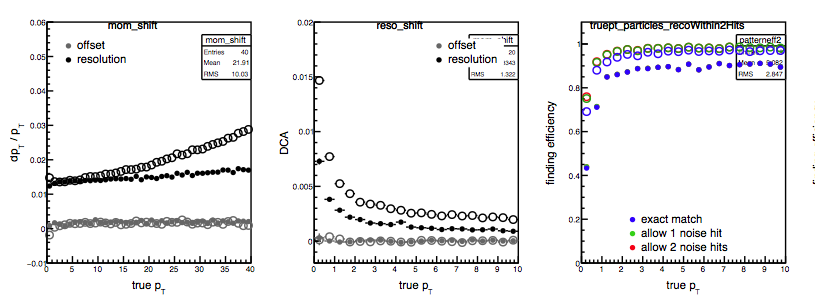
\includegraphics[width=0.9\linewidth]{figs/tracking_performance_reference}
  \caption{Tracking performance for the reference detector
    configuration with an outer TPC tracker and a 3-layer MAPS inner
    tracker. Shown are \pt resolution (left), DCA resolution with
    respect to the primary vertex (center) and track finding
    efficiency (right), all as a function of true particle \pt for
    central \hijing Au+Au collisions.}
  \label{fig:tracking_reference}
\end{figure}

\subsection{Comparison of 2-layer MAPS tracker and VTX pixels} 

Figure~\ref{fig:ups1s_recomass_comparison} shows a comparison of the
$\Upsilon$(1S) mass spectrum from 10,000 Upsilons embedded in central
\hijing events thrown into $\pm1$ unit of rapidity. The two scenarios
are an inner barrel of two MAPS layers (red) and one of two VTX
pixel layers (blue), combined with an ideal outer tracker.  
The VTX pixel efficiencies are 89\% for layer 0 and 76\% for layer 1 and are based
on PHENIX measurements of their performance. While the mass resolution for the 1S state is
only moderately degraded for the VTX pixel simulation, 
the poor efficiency of the VTX pixels causes a nearly 50\% 
drop in Upsilon statistics.
\begin{figure}[hbt]
  \centering
  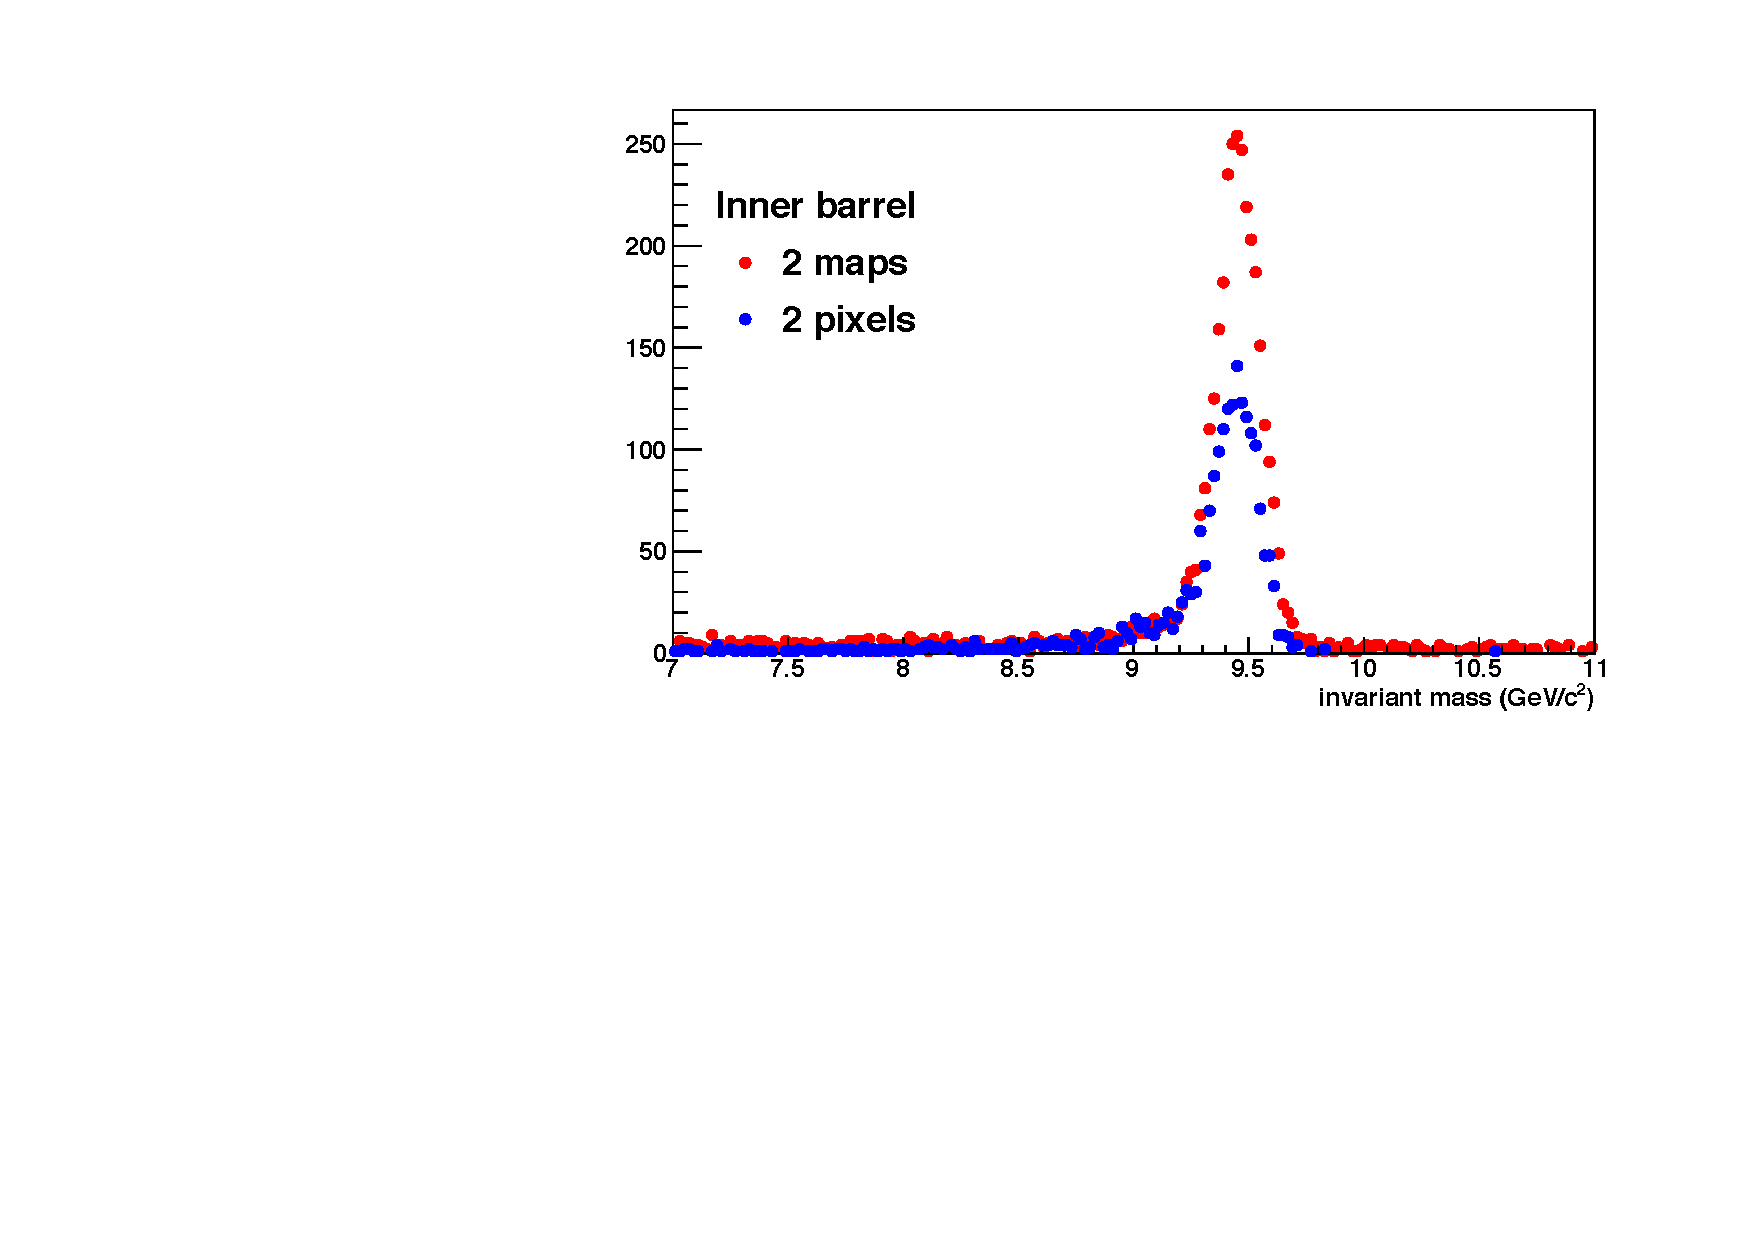
\includegraphics[width=0.5\linewidth]{figs/ups1s_recomass_comparison}
  \caption{Mass spectrum from 10,000 Upsilons embedded in central
\hijing events thrown into $\pm1$ unit of rapidity. The two scenarios
are an inner barrel of two MAPS layers (red) and one of of two VTX
pixel layers (blue).}
\label{fig:ups1s_recomass_comparison}
\end{figure}

\begin{figure}[hbt]
  \centering
  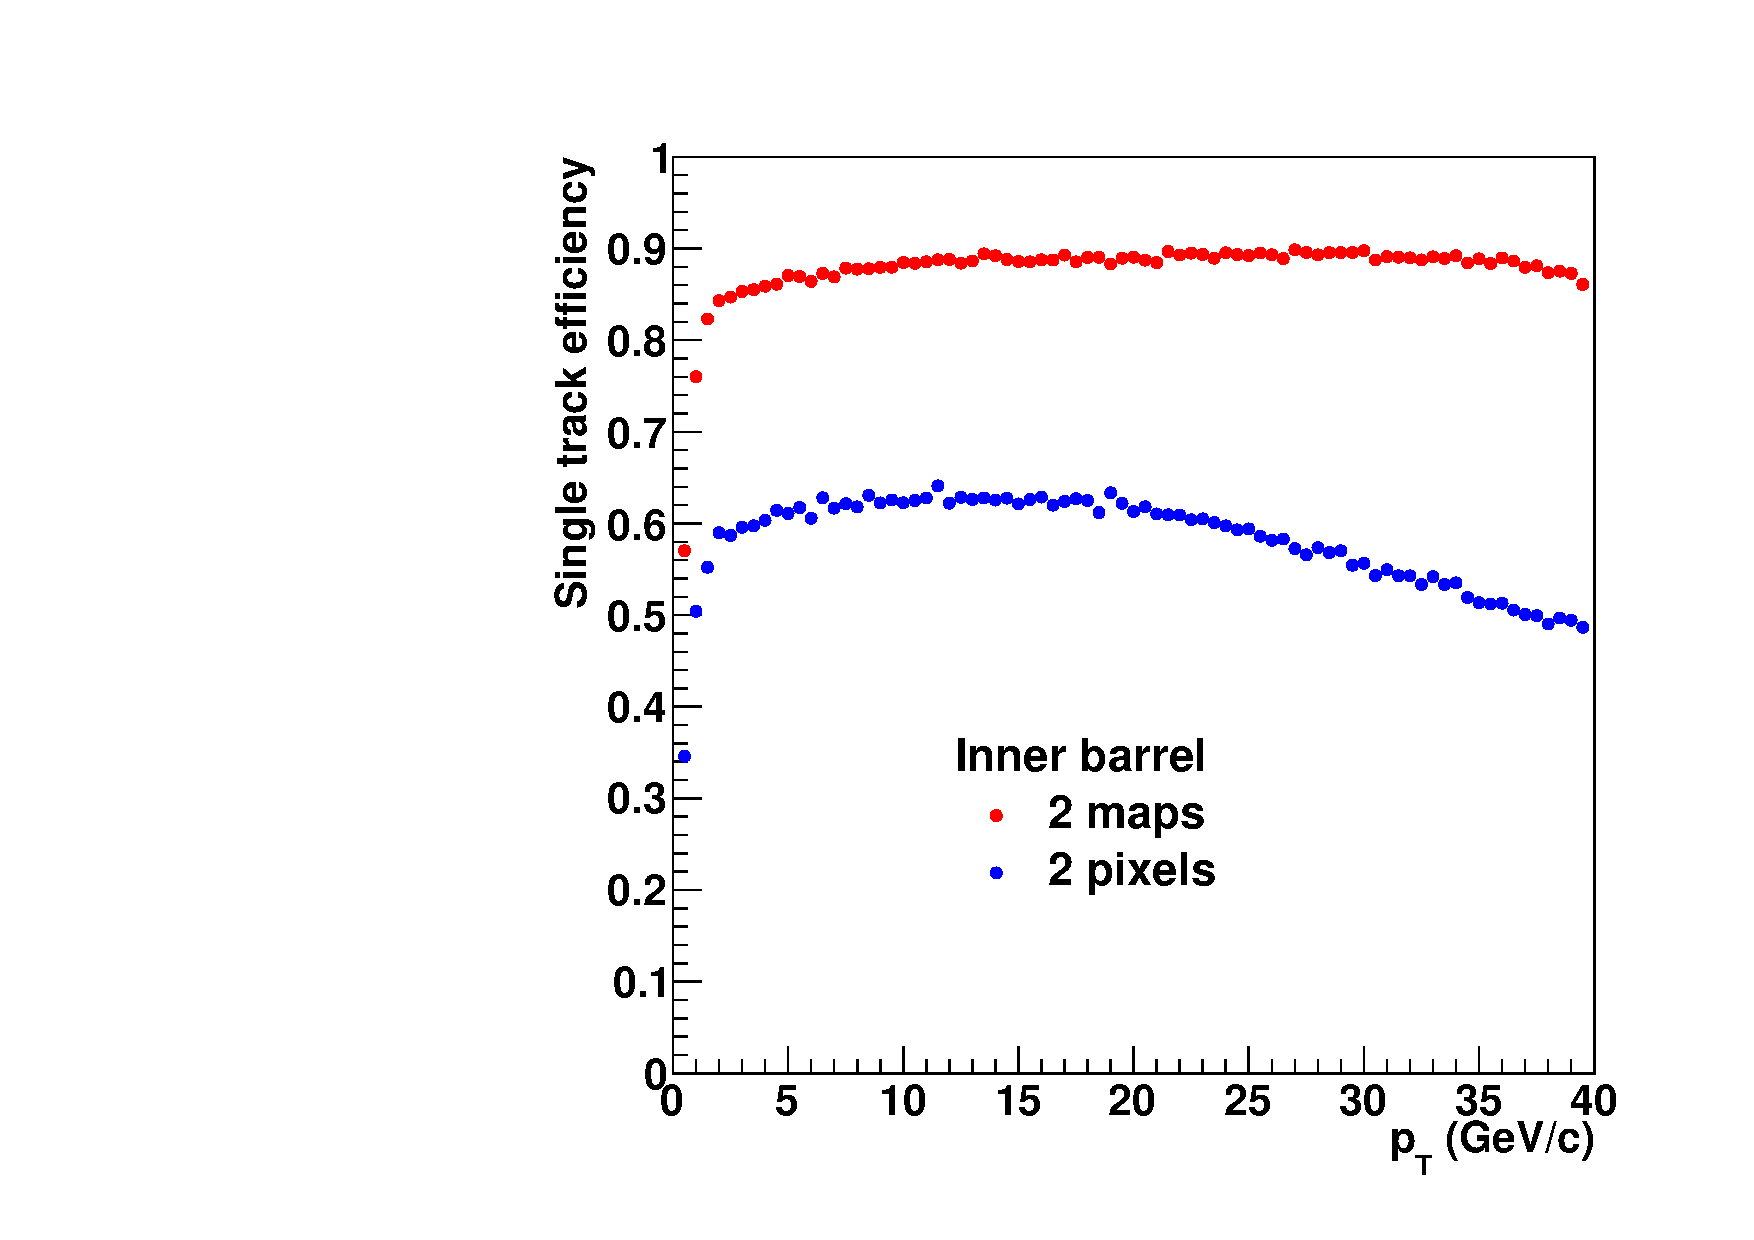
\includegraphics[width=0.4\linewidth]{figs/single_track_efficiency_2maps_vs_2pixels}
  \hspace{0.1\linewidth}  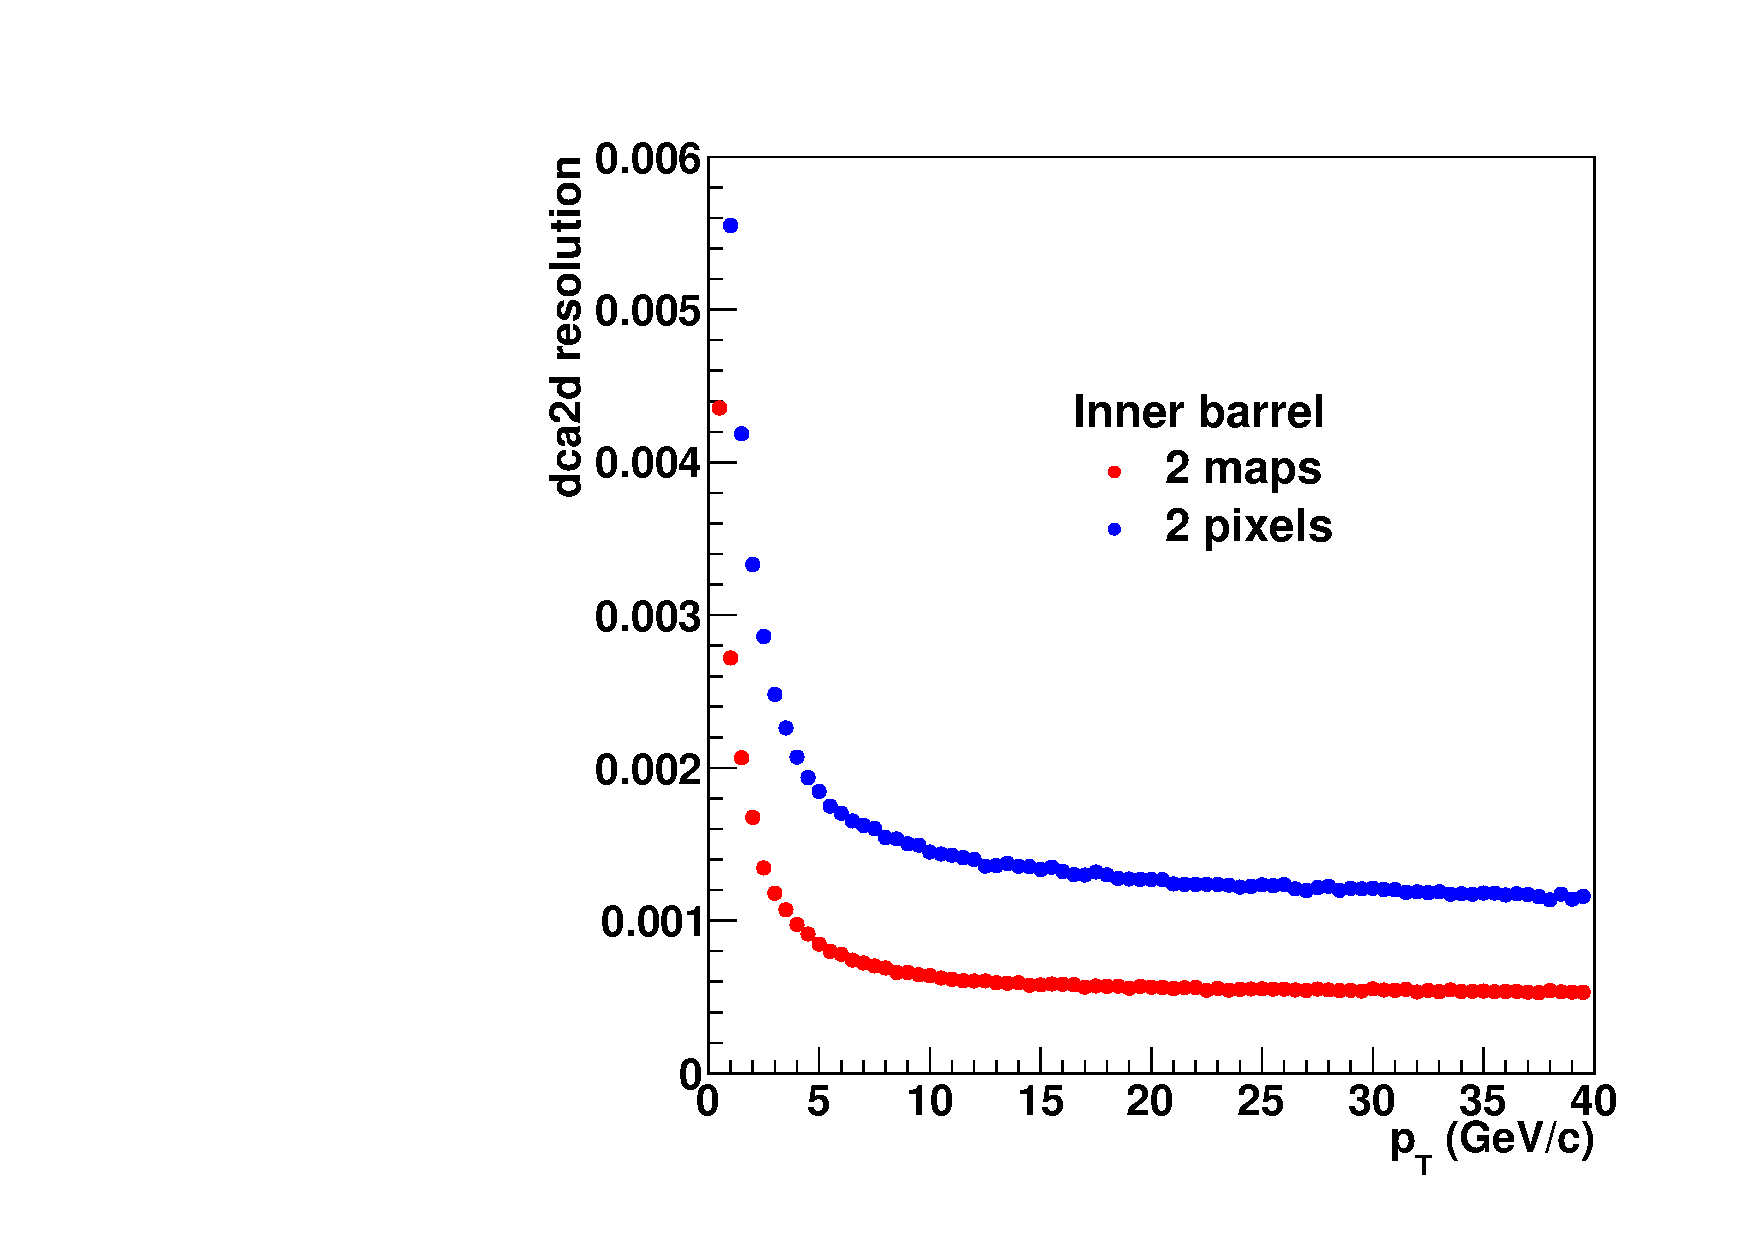
\includegraphics[width=0.4\linewidth]{figs/dca2d_resolution_2maps_vs_2pixels}
  \caption{(Left) Comparison of the single track efficiency as a function of \pt for a two-layer MAPS
  inner tracker (red markers) and a two layer VTX pixel inner tracker (blue markers). 
   (Right) Comparison of the DCA resolution with respect to the primary vertex as a function of \pt for a two-layer MAPS
  inner tracker (red markers) and a two layer VTX pixel inner tracker (blue markers)  }
  \label{fig:2LayerMAPSvsPXL}
\end{figure}

In Fig.~\ref{fig:2LayerMAPSvsPXL} the single track efficiency (left) and DCA resolution (right) for 2-layer MAPS (red markers) 
and VTX pixel (blue markers) inner trackers are compared. The simulations were performed in combination with an ideal outer tracker 
to isolate the performance of the inner tracker. Hits in both inner tracker layers were required. One observes a single track 
efficiency that is about 30\% lower for the VTX pixel inner tracker compared to the MAPS inner tracker, while the DCA resolution 
for the MAPS inner tracker is about a factor of two better. While the lower single track efficiency and DCA resolution of the VTX pixel tracker 
affect statistical and systematic uncertainties of essentially all planned sPHENIX measurements, the impact is particularly
detrimental for the heavy-flavor tagged jet program, which typically relies on identifying multiple tracks with large DCA inside
a jet cone. For a given b-jet purity, the reduced VTX pixel single track efficiency implies a $\approx 50$\% lower b-jet efficiency 
than the MAPS based solution using a selection requiring two large-DCA tracks (for the higher purity 3-track cut, the loss in efficiency
will be correspondingly higher). This performance loss would be in addition to the reduced tagging efficiency due to the lower VTX pixel DCA resoluton.


\section{DAQ and trigger}
\subsection{Minimum bias trigger counter and vertex locator}
We expect that the proposed re-use of an existing vertex detector, or the potential copy of the STAR EPD under construction, will not significantly affect
the physics performance for any of the benchmark measurements.
\subsection{Offline event building}
We expect that the proposed change of event-building strategy will not significantly affect the physics performance for any of the benchmark measurements,
although it will likely introduce an additional latency in the initial offline reconstruction that remains to be evaluated.

\section{Interference of calorimeter options}
\begin{figure}[hbt]
  \centering
  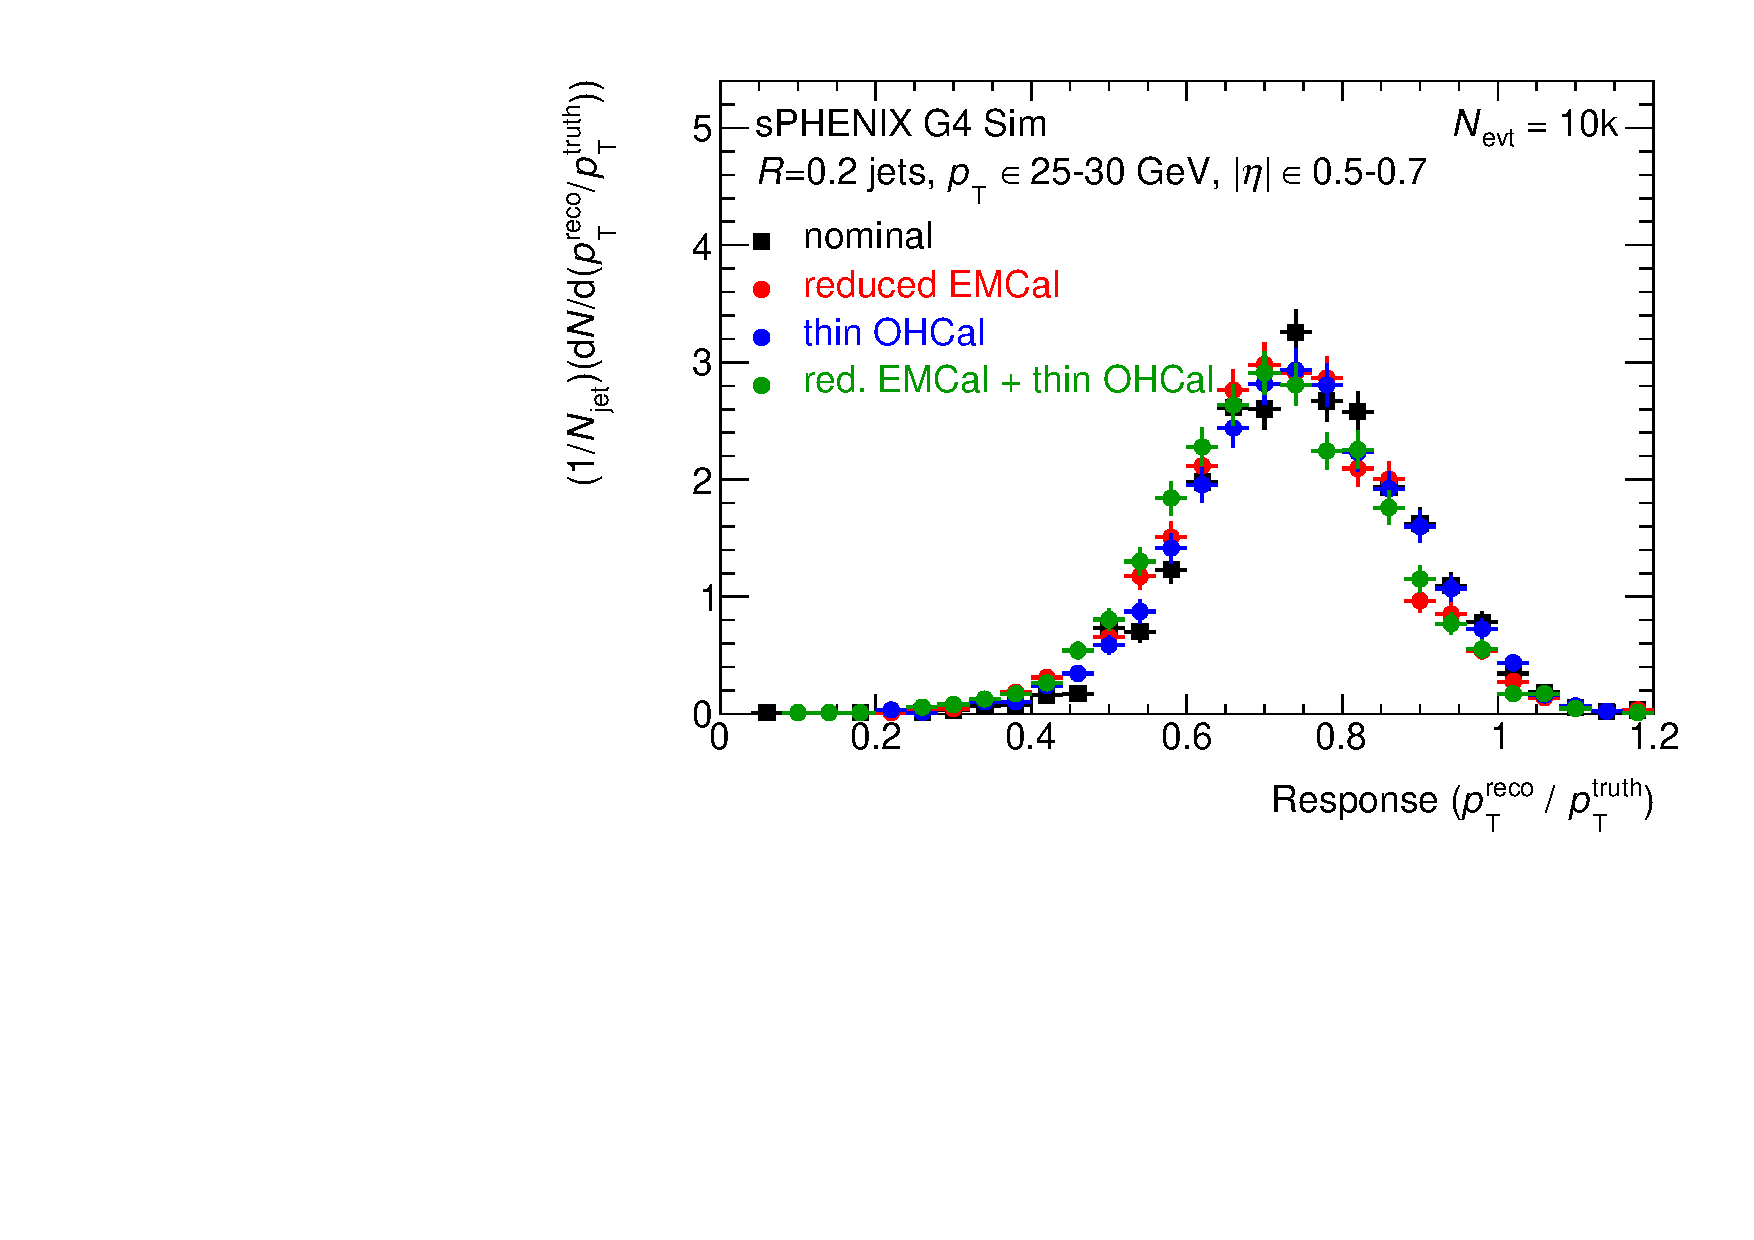
\includegraphics[width=0.4\linewidth]{figs/h1_etascan_response_ETA1}
  \hspace{0.1\linewidth}  
  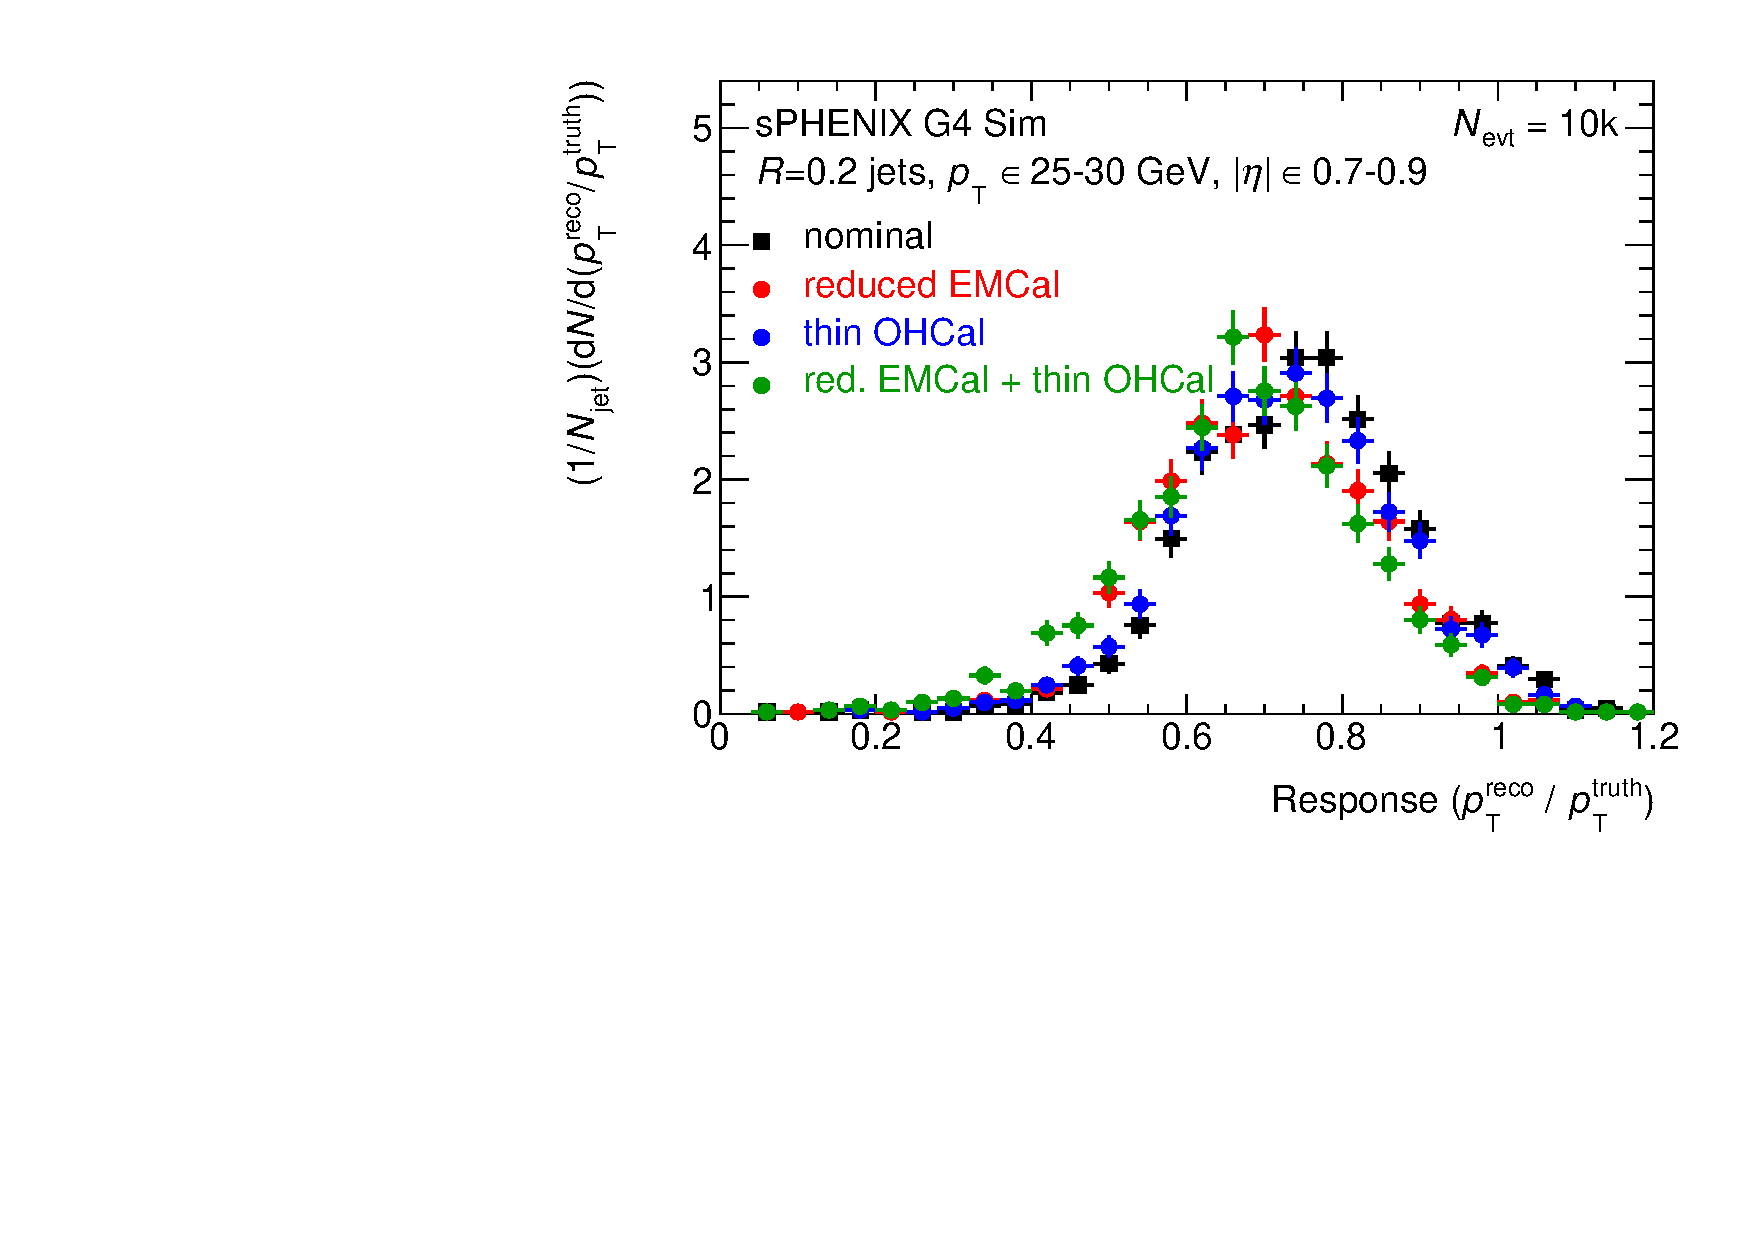
\includegraphics[width=0.4\linewidth]{figs/h1_etascan_response_ETA2}
  \caption{Jet response for low \pt jets for four calorimeter configurations:
   nominal (black markers), reduced EMCal acceptance (red), thinned outer HCAL (blue) and a combination
   reduced acceptance EMCal and thinned outer HCal (green markers) for two different jet pseudorapidity regions: $0.5 < |\eta| < 0.7$ (left) and 
$0.7 < |\eta| < 0.9$ (right) }
  \label{fig:JetResponse25GeV_CaloStackVariants_Nevt20k}
\end{figure}
Most of the de-scoping options discussed in this document can in good approximation be evaluated independently and combined to achieve certain levels of savings 
and physics performance. This is not the case when considering combinations of some of the HCAL and EMCal options with respect to the 
jet reconstruction performance. This includes in particular:
\begin{itemize}
\item Thinning of the outer HCAl by $\approx 20$~cm
\item Removal of the inner HCal
\item Reduction of the EMCal acceptance to $|\eta| < 0.6$
\end{itemize}
Each of these options in essence removes about one interaction length from the calorimeter system. Our simulations show that for a 
change by one interaction length the resulting change in calorimeter response is comparable to the typical
systematic uncertainties achieved in such measurements. Combining two such changes in the same acceptance region however leads to 
a loss of energy containment that significantly degrades performance. An example of this is shown for the combined effect of 
outer HCAL thinning and reduced EMCal acceptance in Fig.~\ref{fig:JetResponse25GeV_CaloStackVariants_Nevt20k} (right), for jets with
$25 < \pt < 30$~GeV/c and $0.7 < |\eta| < 0.9$, which fall outside the reduced EMCal acceptance. While the
performance compared to the nominal configuration is acceptable for either the thinned outer HCal (blue markers) or the reduced acceptance EMCal (red markers),
the combination of both changes, shown as green markers, leads to a jet energy response that is shifted by more than 10\% compared to the nominal 
configuration and a wide tail that will limit the accuracy with which the response function could be unfolded 
to yield high precision jet spectra. As a consequence, a combination of any of the thinning options is highly detrimental when aiming for 
accurate jet spectra measurements.

